\documentclass[10pt,a4paper]{article}
\usepackage[margin=2.2cm]{geometry}
\usepackage{fontspec}
\usepackage{kotex}
\setmainfont{Apple SD Gothic Neo}
\setsansfont{Apple SD Gothic Neo}
\usepackage{amsmath,amssymb}
\usepackage{graphicx}
\usepackage{booktabs}
\usepackage{caption}
\usepackage[dvipsnames]{xcolor}
\usepackage[colorlinks=true,linkcolor=MidnightBlue,citecolor=MidnightBlue,
            urlcolor=MidnightBlue]{hyperref}
\usepackage{titlesec}
\titleformat{\section}{\large\bfseries}{\thesection}{0.6em}{}
\titleformat{\subsection}{\normalsize\bfseries}{\thesubsection}{0.5em}{}
\captionsetup{font=small,labelfont=bf}
\setlength{\parskip}{0.35em}
\setlength{\parindent}{0pt}

\usepackage{mdframed}
\newmdenv[linewidth=0.4pt,linecolor=gray!60,backgroundcolor=gray!5,
          innertopmargin=6pt,innerbottommargin=6pt,skipabove=8pt,skipbelow=8pt]{claimbox}
\newcommand{\claim}[2]{\begin{claimbox}\textbf{주장.} #1\par\smallskip
  \textcolor{gray!70}{\textbf{반증 조건.} #2}\end{claimbox}}

\title{\bfseries 옳은 값, 틀린 이름\\[2pt]
\large 아이돌 제목 짝 수리 --- 두 순서의 화해}
\author{월드모델 실험실 · 노트 $810$}
\date{2026-08-07}
\begin{document}\maketitle

\section{한 줄}

논문 $172$ 가 남긴 빚(아이돌 제목 $81$ 대 판 $173$)의 뿌리를 캤다.
\texttt{titles(아이돌)} 의 id 순서가 \texttt{idol\_axes.json}($81$키)에서 오는데
판의 아이돌 행은 \texttt{idolset.\_rows}($173$행 · 한터 $79$ $+$ 추가 $94$)를
따른다 --- \textbf{값은 record\_id 로 옳게 붙었고 순서가 달라, 창구가 위치로
붙인 제목-행 짝이 틀렸다.}

수리: 제목의 id 순서를 \textbf{판과 같은 원천}(\texttt{idolset.\_rows})으로.
격자 $5/5$ --- 길이 $173$ 일치 · \textbf{전수 짝 검사 $0$ 불일치} · 다른 도메인
불변 · 재굽기 후 유보 제목 $25 \to 51$ 전부 · 무효화 유지.

\begin{figure}[t]\centering
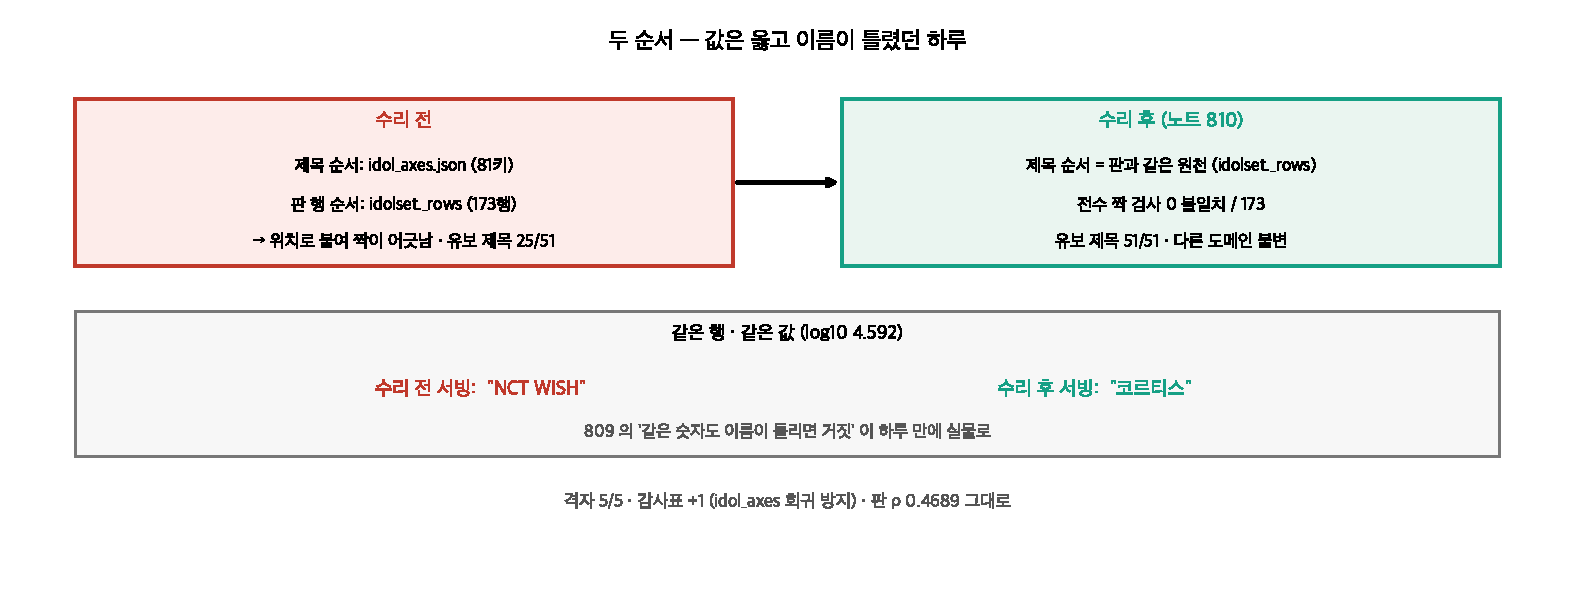
\includegraphics[width=0.95\textwidth]{figs/name.pdf}
\caption{같은 행, 같은 값($4.592$) --- 수리 전엔 ``NCT WISH'', 후엔 ``코르티스''.}
\end{figure}

\section{하루 만에 돌아온 문장}

\claim{\textbf{어제의 서빙은 틀린 이름을 내보내고 있었다.} \texttt{absolute}
(아이돌)의 값(log$10$ $4.592$)은 내내 옳았는데 그 행의 이름이 ``NCT WISH''로
표시됐다 --- 실제는 ``코르티스''다. 논문 $172$ 가 적은 \emph{``같은 숫자도
이름이 틀리면 거짓이 된다''}가 \textbf{하루 만에 실물로 돌아왔다.} 챔피언 점수와는
무관하다(노트 $806$: 같은 $X$ 에서의 부류 차이가 아이돌 결손의 원인 --- A·M 은
이 수리와 무관하게 동일).}
{감사표에 회귀 방지를 걸었다(id 순서가 \texttt{idol\_axes} 로 돌아가면 잡힌다).
남는 위험: \texttt{idolset.\_rows} 의 필터가 바뀌면 제목과 판이 \emph{함께}
움직여야 하는데 둘이 같은 함수를 부르므로 구조적으로 같이 간다 --- 두 군데
거름망이 갈라지던 노트 $359$ 의 병을 원천 공유로 피했다.}

\section{T$1$ 이 닫혔다}

아이돌 배선 미결이 이것으로 닫혔고, \textbf{T$1$ 의 측정 가능 갈래가 소진됐다}
--- 남은 셋(KOBIS $12$도메인 챌린저 재측정 · 두꺼운 텍스트의 A$1$ 재시험 · 보조
헤드 서빙 승격 절차)은 전부 \textbf{수집 또는 사람 승인이 문이다.} 판 $\rho$
$0.4689$ 그대로.

\end{document}
